\documentclass[11pt,a4paper]{article}

\usepackage[utf8]{inputenc}
\usepackage[T1]{fontenc}
\usepackage{lmodern}
\usepackage[margin=2.5cm]{geometry}
\usepackage{graphicx}
\usepackage{booktabs}
\usepackage{amsmath}
\usepackage{float}
\usepackage{xcolor}
\usepackage{listings}
\usepackage{caption}
\usepackage{microtype}
\usepackage[hidelinks]{hyperref}

\graphicspath{{../results/figures/}}
\lstset{basicstyle=\ttfamily\footnotesize, breaklines=true, frame=single, backgroundcolor=\color{black!3}, columns=fullflexible}
\renewcommand{\arraystretch}{1.1}

\title{\textbf{CFD Flow Prediction Benchmarking Suite}\\[4pt]
\large Reproducible datasets, standard evaluation tools and an online leaderboard}
\author{Pierrick Vignal\\[6pt]
\small Master in High Performance Computing, Universidade da Coru\~na\\
\small Supervisors: Emilio J.\ Padr\'on Gonz\'alez and Omar A.\ Mures}
\date{Working draft, November 2026}

\begin{document}
\maketitle

\begin{abstract}
Machine-learning models that predict fluid flows are rarely compared on common data: each paper uses its own cases, metrics and code, so results are hard to reproduce and to compare. This work presents a small benchmarking suite that covers the whole loop: a versioned dataset with fixed training, interpolation and extrapolation splits; standard preprocessing and post-processing tools; baseline models; and a web platform that scores submitted predictions and ranks them on a leaderboard. The reference data are generated by a lattice Boltzmann solver for the 2D flow past a circular cylinder (Reynolds numbers 30 to 180); the task is to predict the time-averaged velocity field from the Reynolds number. Seven baselines are evaluated. Linear interpolation obtains a relative L2 error of 0.031 in interpolation and 0.054 in extrapolation; polynomial regression of POD coefficients is accurate inside the training range but diverges outside it (0.219). The solver overestimates the Strouhal number by 16\% in the dataset geometry because of confinement (8\% in a domain twice as wide). A performance study shows that the CPU data generation scales poorly (best speedup 1.65 with four processes) and that a GPU brings a 17x to 31x speedup only on grids much larger than the dataset grid. The main limitation is that the data are simulated, not experimental.
\end{abstract}

\newpage
\tableofcontents
\newpage

%--------------------------------------------------------------------
\section{Introduction}
\subsection{Motivation}
Computational fluid dynamics (CFD) simulations are expensive, which motivates data-driven surrogate models that predict flow fields in a fraction of the time. The field suffers from a lack of standard benchmarks: models are rarely tested on common datasets and the code and data are often not shared. This slows innovation, weakens reproducibility and makes fair comparison between methods difficult.

\subsection{Objectives}
The thesis proposal asks for a benchmarking suite with four components:
\begin{enumerate}
  \item a standardized, validated dataset repository for evaluating CFD prediction models;
  \item standard tools for preprocessing CFD data, especially image-based flow representations;
  \item post-processing pipelines for consistent evaluation and comparison;
  \item an online application with dataset access, documentation and a leaderboard.
\end{enumerate}
This report describes the implementation of these components in the open-source package \texttt{cfdbench}\footnote{\url{https://github.com/Gotrone/TFM}} and the experiments carried out with it.

\subsection{Scope and honesty about what was done}
\textbf{The reference data are simulated by a solver written for this work, not experimental measurements.} The proposal mentions experimentally validated datasets; these were not integrated. The suite is therefore a working, tested pipeline with a self-generated 2D laminar benchmark, designed so that real datasets can be plugged in later. Section~\ref{sec:limits} lists the limitations in detail.

\subsection{Contributions}
\begin{itemize}
  \item a versioned cylinder-flow benchmark with three splits (train, interpolation, extrapolation) and a checksum;
  \item a regularized lattice Boltzmann solver with CPU (NumPy) and GPU (CuPy) back ends;
  \item preprocessing, metrics, seven baseline models (including a small neural network) and a SQLite leaderboard;
  \item a FastAPI web platform with server-side scoring, an optional API key and a rate limit;
  \item a partial validation of the solver (Strouhal number), a performance study of the data generation (processes, CPU vs.\ GPU) and SLURM job scripts;
  \item 24 automated tests, continuous integration and a Docker image.
\end{itemize}

%--------------------------------------------------------------------
\section{Background and related work}
\paragraph{ML benchmarks for fluid flows.} CFDBench~\cite{luo2023cfdbench} provides a large collection of canonical cases (more than 300\,000 frames over four geometries) to evaluate neural operators. FlowBench~\cite{tali2024flowbench} adds more than 10\,000 samples of complex 2D and 3D flows with several physical variables. The FDA nozzle and blood pump benchmarks provide experimental data reproduced by several laboratories and serve as a reference for validating CFD in physiological conditions. These resources motivate the present design but are not used here.

\paragraph{Deep learning for the cylinder wake.} Lee and You~\cite{lee2019data} showed that convolutional and generative networks can predict the unsteady flow over a circular cylinder, including Reynolds numbers unseen during training, which illustrates the potential of surrogate models and the need to test them outside the training range.

\paragraph{Tools.} FluidFoam~\cite{fluidfoam} reads OpenFOAM data in Python and is the planned entry point for real CFD datasets.

\paragraph{Lattice Boltzmann method.} The lattice Boltzmann method (LBM) simulates weakly compressible flows with local collision and nearest-neighbour streaming steps~\cite{kruger2017lbm}. It is simple to implement and to parallelize, which makes it a good choice to generate reference data on any machine. The regularized variant~\cite{latt2006regularized} improves stability at low viscosity.

%--------------------------------------------------------------------
\section{Benchmark design}
\subsection{Task}
The flow past a circular cylinder in a channel is characterized by the Reynolds number
\begin{equation}
  Re = \frac{u_{\mathrm{in}} D}{\nu},
\end{equation}
where $u_{\mathrm{in}}$ is the inlet velocity, $D$ the cylinder diameter and $\nu$ the kinematic viscosity. The wake changes with $Re$: for an unbounded cylinder, vortex shedding starts around $Re\approx 47$ and the mean recirculation bubble shortens as $Re$ increases. The benchmark task is:

\begin{quote}
\emph{Given $Re$, predict the time-averaged velocity field $(u,v)$ on a $200\times72$ grid} (velocities divided by $u_{\mathrm{in}}$).
\end{quote}

\subsection{Splits}
Samples are split by Reynolds number so that generalization can be evaluated separately between and beyond the training points (Table~\ref{tab:splits}).

\begin{table}[H]
\centering
\caption{Dataset splits (version 2.0, 27 simulations).}\label{tab:splits}
\begin{tabular}{lp{7.3cm}l}
\toprule
Split & Reynolds numbers & Purpose\\
\midrule
\texttt{train} & 40, 60, 80, 100, 120, 140 & fit the models\\
\texttt{test\_interp} & 45, 50, 55, 65, 70, 75, 85, 90, 95, 105, 110, 115, 125, 130, 135 & between training points\\
\texttt{test\_extrap} & 30, 35, 150, 160, 170, 180 & outside the training range\\
\bottomrule
\end{tabular}
\end{table}

\begin{figure}[H]
\centering
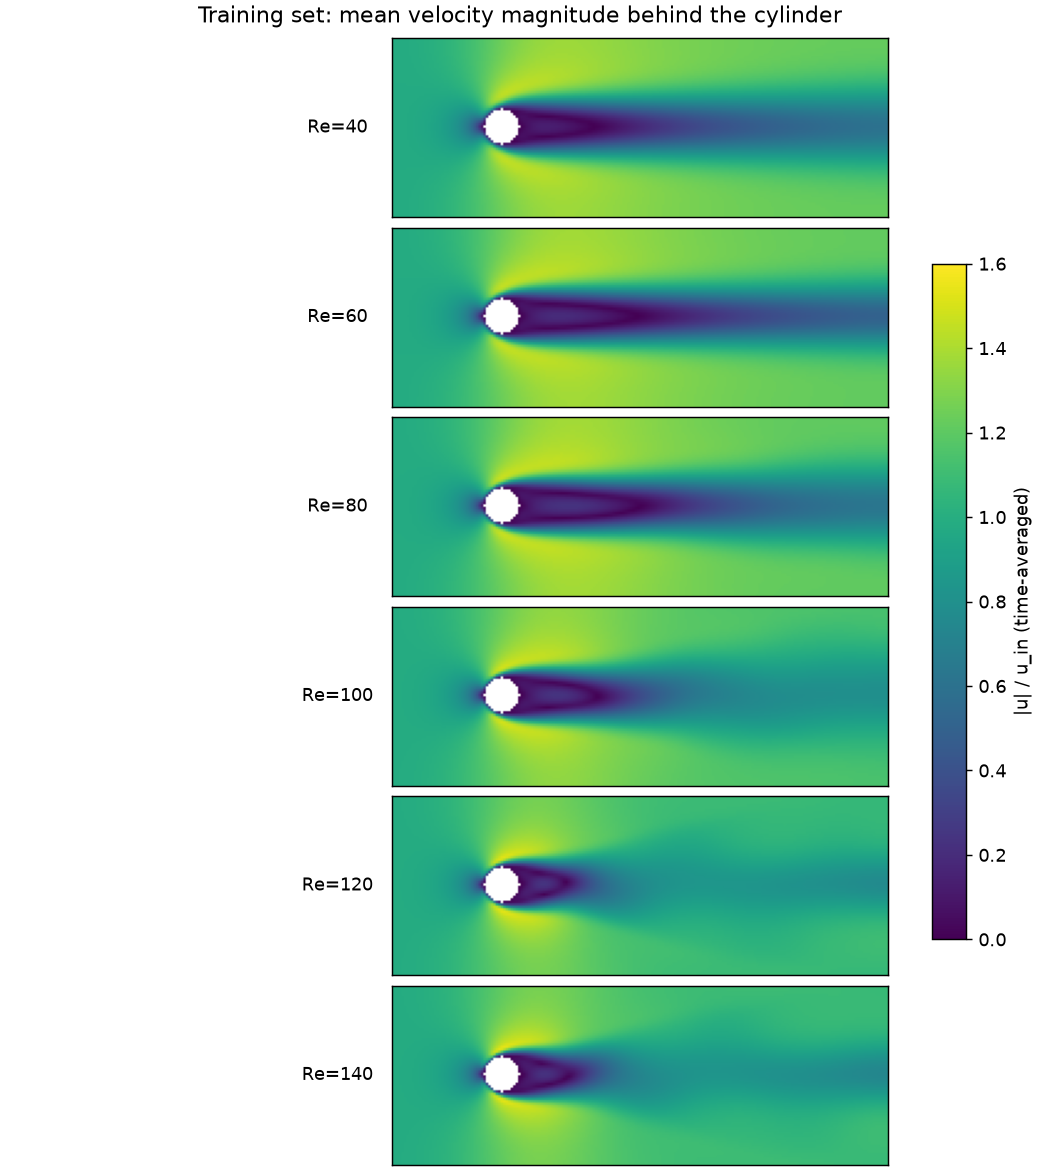
\includegraphics[width=0.8\textwidth]{dataset_overview.png}
\caption{Mean velocity magnitude of the six training cases. The recirculation zone behind the cylinder shortens as $Re$ increases.}
\end{figure}

\subsection{Metrics}
All metrics are computed on fluid cells only (the cylinder is excluded) and averaged over the samples of a split. With $\hat{\mathbf u}$ the prediction and $\mathbf u$ the truth:
\begin{align}
  \mathrm{rel\_L2} &= \frac{\lVert \hat{\mathbf u}-\mathbf u\rVert_2}{\lVert \mathbf u\rVert_2} \quad\text{(ranking metric)},\\
  \mathrm{MSE} &= \operatorname{mean}\big[(\hat{\mathbf u}-\mathbf u)^2\big], \qquad \mathrm{MAE}=\operatorname{mean}\big[|\hat{\mathbf u}-\mathbf u|\big].
\end{align}
Three more metrics are reported: the largest cell error (\texttt{max\_abs}), the relative L2 error restricted to the wake downstream of the cylinder (\texttt{wake\_rel\_l2}), and the RMS divergence of the prediction (\texttt{div\_rms}), a physical-consistency check since the mean flow of an incompressible fluid is divergence-free.

\subsection{Platform architecture}
\begin{figure}[H]
\centering
\begin{lstlisting}
cfdbench/
  lbm.py            LBM solver (CPU/GPU)
  dataset.py        generation, splits, storage, checksum
  preprocessing.py  normalization, resampling, image export
  metrics.py        evaluation metrics
  models.py         Model interface, registry, 7 baselines
  benchmark.py      fit / predict / score loop
  leaderboard.py    SQLite ranking
  web/              FastAPI application and front end
  scaling.py        performance studies
  validation.py     Strouhal-number check
\end{lstlisting}
\caption{Package structure.}
\end{figure}
Participants download the training split from the web application; it contains the training fields and only the Reynolds numbers of the test splits, never the test fields. They upload predictions as an \texttt{.npz} file, which the server scores and adds to the leaderboard.

%--------------------------------------------------------------------
\section{Implementation}
\subsection{Reference solver}
The solver uses the D2Q9 lattice with a regularized BGK collision. The relaxation time is related to the viscosity by $\nu = c_s^2(\tau - \tfrac12)$ with $c_s^2 = 1/3$. The boundary conditions are a uniform inlet (equilibrium distribution), a zero-gradient outlet, periodic top and bottom boundaries and bounce-back on the cylinder. The grid is $200\times72$ with a cylinder diameter of 14 cells (blockage $D/n_y = 19.4\%$) and an inlet velocity of 0.08 in lattice units. Each case runs 10\,000 warm-up steps and averages 3\,200 further steps. The same code runs on the CPU (NumPy) or on an NVIDIA GPU (CuPy) through a common array module; float32 or float64 can be selected.

\subsection{Preprocessing}
A \texttt{Standardizer} normalizes each channel using statistics computed on fluid cells of the training set only, sets solid cells to zero and is exactly invertible. Other tools provide block-average downsampling, cropping of a region of interest and conversion of a scalar field to an RGB image for vision models.

\subsection{Baseline models}
Table~\ref{tab:models} lists the baselines. The reduced-order models first compute a proper orthogonal decomposition (POD, via SVD) of the standardized training fields, keep five modes, regress the modal coefficients on $Re$, and reconstruct the field.

\begin{table}[H]
\centering
\caption{Baseline models.}\label{tab:models}
\begin{tabular}{ll}
\toprule
Model & Description\\
\midrule
\texttt{freestream} & uniform flow $u=1$, $v=0$ (no obstacle effect)\\
\texttt{mean} & average training field\\
\texttt{nearest} & field of the closest training $Re$\\
\texttt{linear} & pixel-wise linear interpolation in $Re$ (clamped outside the range)\\
\texttt{pod-poly} & POD + cubic polynomial regression of the coefficients\\
\texttt{pod-gp} & POD + Gaussian-process regression\\
\texttt{pod-mlp} & POD + small neural network (MLP, two layers of 16 units)\\
\bottomrule
\end{tabular}
\end{table}

\subsection{Web platform and reproducibility}
The FastAPI application exposes the dataset description and training split, a ranked leaderboard (by any metric) and a submission endpoint. Uploads are limited to 25\,MB, names are validated, an optional API key protects submissions and a per-IP rate limit (10 per hour by default, kept in memory) slows abuse. The package is covered by 24 automated tests (solver, preprocessing, metrics, models, API), a GitHub Actions workflow runs the linter and the tests on Python 3.10 and 3.12, and a Docker image bundles the dataset and the pre-filled leaderboard.

%--------------------------------------------------------------------
\section{Experiments and results}
\subsection{Solver validation}
The shedding frequency was measured with a probe in the wake and expressed as a Strouhal number $St = fD/u_{\mathrm{in}}$. It is compared with the fit $St = 0.2665 - 1.018/\sqrt{Re}$ for unconfined cylinders~\cite{williamson1998series}. Table~\ref{tab:strouhal} shows that the solver overestimates $St$, and that the error roughly halves when the blockage is halved, so confinement explains a large part of it. The rest may come from the coarse resolution (14 cells per diameter), which was not tested. Drag was not validated and no grid-convergence study was made. The dataset therefore describes a \emph{confined} cylinder flow.

\begin{table}[H]
\centering
\caption{Strouhal number measured vs.\ reference.}\label{tab:strouhal}
\begin{tabular}{rllrrr}
\toprule
$Re$ & Domain & Blockage & $St$ measured & $St$ reference & Error\\
\midrule
100 & $200\times72$ (dataset) & 19.4\% & 0.191 & 0.165 & +16\%\\
100 & $200\times144$ & 9.7\% & 0.178 & 0.165 & +8\%\\
140 & $200\times72$ (dataset) & 19.4\% & 0.203 & 0.180 & +12\%\\
140 & $200\times144$ & 9.7\% & 0.191 & 0.180 & +6\%\\
\bottomrule
\end{tabular}
\end{table}

\subsection{Baseline results}
Table~\ref{tab:results} gives the relative L2 error of each model on the test splits, and Figure~\ref{fig:error} shows the error for every test Reynolds number.

\begin{table}[H]
\centering
\caption{Relative L2 error (lower is better), mean over the test cases of each split.}\label{tab:results}
\begin{tabular}{lrr}
\toprule
Model & \texttt{test\_interp} (15 cases) & \texttt{test\_extrap} (6 cases)\\
\midrule
\texttt{linear} & \textbf{0.031} & 0.054\\
\texttt{pod-mlp} & 0.032 & 0.084\\
\texttt{pod-gp} & 0.035 & 0.120\\
\texttt{pod-poly} & 0.036 & 0.219\\
\texttt{nearest} & 0.044 & 0.054\\
\texttt{mean} & 0.090 & 0.121\\
\texttt{freestream} & 0.306 & 0.246\\
\bottomrule
\end{tabular}
\end{table}

\begin{figure}[H]
\centering
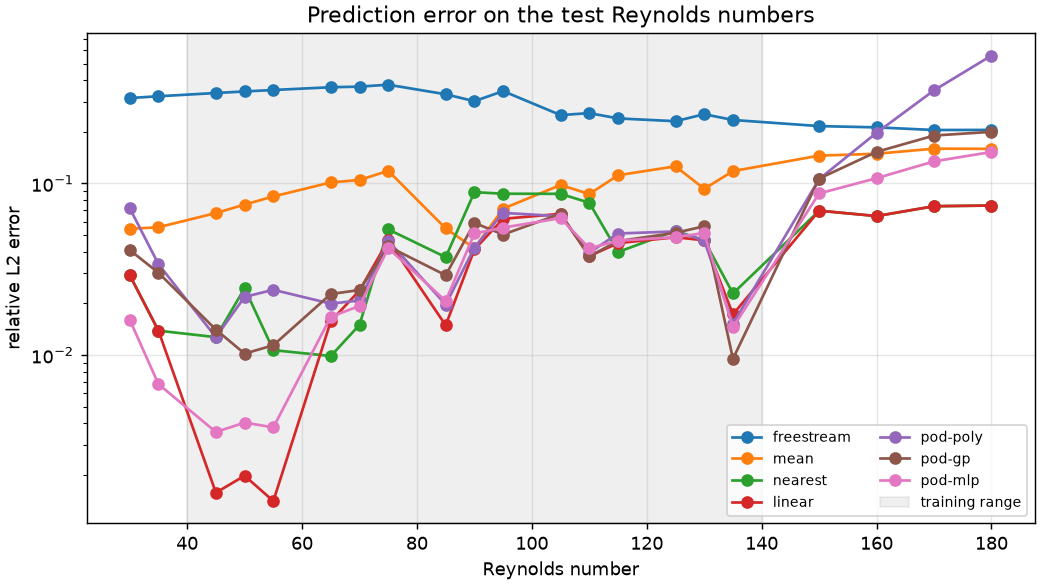
\includegraphics[width=0.85\textwidth]{error_vs_reynolds.png}
\caption{Relative L2 error against the Reynolds number (results of the first dataset version, with fewer test points; the ranking is the same as in Table~\ref{tab:results}).}\label{fig:error}
\end{figure}

\begin{figure}[H]
\centering
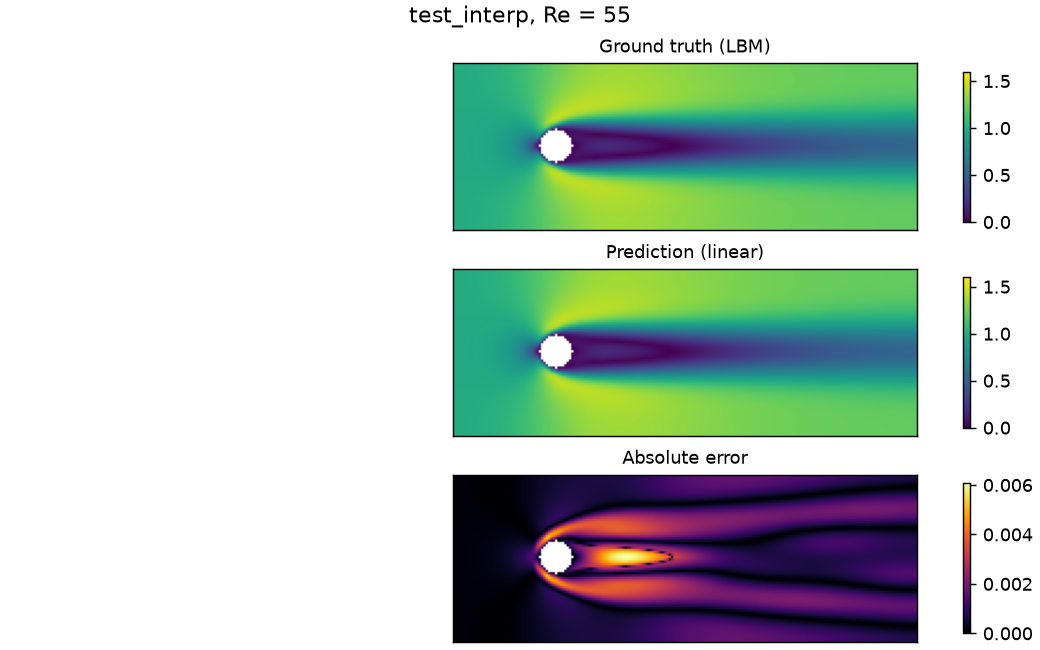
\includegraphics[width=0.85\textwidth]{comparison_linear_interp.png}
\caption{Ground truth, prediction of the best interpolation model and absolute error for one test case.}
\end{figure}

\paragraph{Observations.}
\begin{itemize}
  \item Interpolation is easy for simple methods on this smooth family of flows; the differences between the four best models are small compared with the sizes of the test sets.
  \item Polynomial regression of POD coefficients is accurate inside the training range and diverges outside it (0.219, worse than the average field). The Gaussian process and the neural network degrade less, and clamped methods (\texttt{linear}, \texttt{nearest}) degrade gracefully, but no baseline truly extrapolates.
  \item The divergence of all non-trivial predictions is of the same order ($\approx 10^{-3}$), so the metric does not discriminate between them on this dataset.
\end{itemize}

\subsection{Performance of the data generation}
Hardware: AMD Ryzen 7 4800H (8 cores, 16 threads), NVIDIA GTX 1660 Ti (6\,GB), Windows. Each configuration was measured once.

\paragraph{Process scaling.} Sixteen short simulations (1\,000 steps) were run with 1 to 16 worker processes (Table~\ref{tab:procs}, Figure~\ref{fig:procs}). The scaling is poor: the best speedup is 1.65 with four processes and it decreases beyond. A RAM-to-RAM copy test shows that the per-process memory bandwidth falls from 18\,GB/s (one process) to 4.5\,GB/s (sixteen), which supports the hypothesis that the solver is memory-bandwidth bound. It does not explain everything, since total bandwidth still grows about fourfold; hyper-threading, process start-up time and the shared cache probably contribute and were not isolated.

\begin{table}[H]
\centering
\caption{Strong scaling of the CPU data generation.}\label{tab:procs}
\begin{tabular}{rrrr}
\toprule
Workers & Time (s) & Speedup & Efficiency\\
\midrule
1 & 83.4 & 1.00 & 1.00\\
2 & 53.1 & 1.57 & 0.79\\
4 & 50.6 & 1.65 & 0.41\\
8 & 61.6 & 1.35 & 0.17\\
16 & 65.1 & 1.28 & 0.08\\
\bottomrule
\end{tabular}
\end{table}

\begin{figure}[H]
\centering
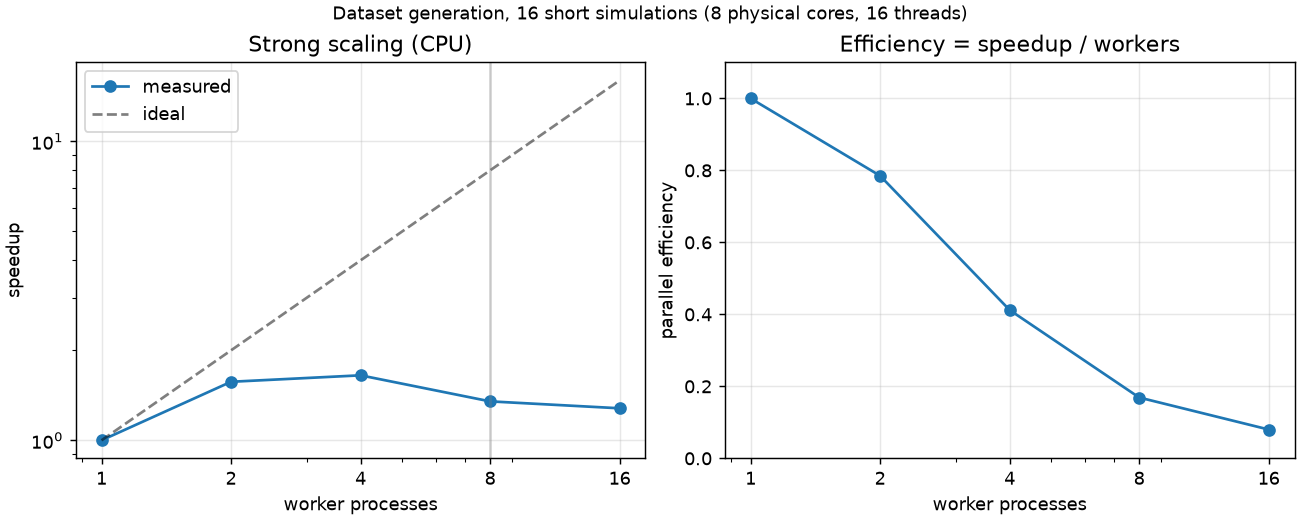
\includegraphics[width=0.9\textwidth]{scaling_processes.png}
\caption{Speedup and parallel efficiency of the CPU data generation.}\label{fig:procs}
\end{figure}

\paragraph{CPU vs.\ GPU.} Throughput in million lattice updates per second (MLUPS) was measured for grids from the dataset size up to $3200\times1152$ (Table~\ref{tab:gpu}, Figure~\ref{fig:gpu}). On the dataset grid the GPU brings nothing, because a step is limited by the latency of launching about one hundred small kernels. From $400\times144$ on the GPU wins, reaching about 17x (float64) and 31x (float32) the throughput of one CPU process on the largest grid. A copy test reaches 268\,GB/s on the GPU (specification: 288), so the 53\,MLUPS obtained are far from what the hardware allows: the array temporaries of the NumPy/CuPy style waste bandwidth.

\begin{table}[H]
\centering
\caption{Solver throughput (MLUPS, higher is better).}\label{tab:gpu}
\begin{tabular}{lrrr}
\toprule
Grid & CPU float64 & GPU float64 & GPU float32\\
\midrule
$200\times72$ (dataset) & 2.9 & 2.6 & 3.2\\
$400\times144$ & 1.7 & 12.1 & 12.8\\
$800\times288$ & 1.8 & 23.3 & 35.9\\
$1600\times576$ & 1.7 & 29.9 & 51.7\\
$3200\times1152$ & 1.7 & 30.8 & 53.6\\
\bottomrule
\end{tabular}
\end{table}

\begin{figure}[H]
\centering
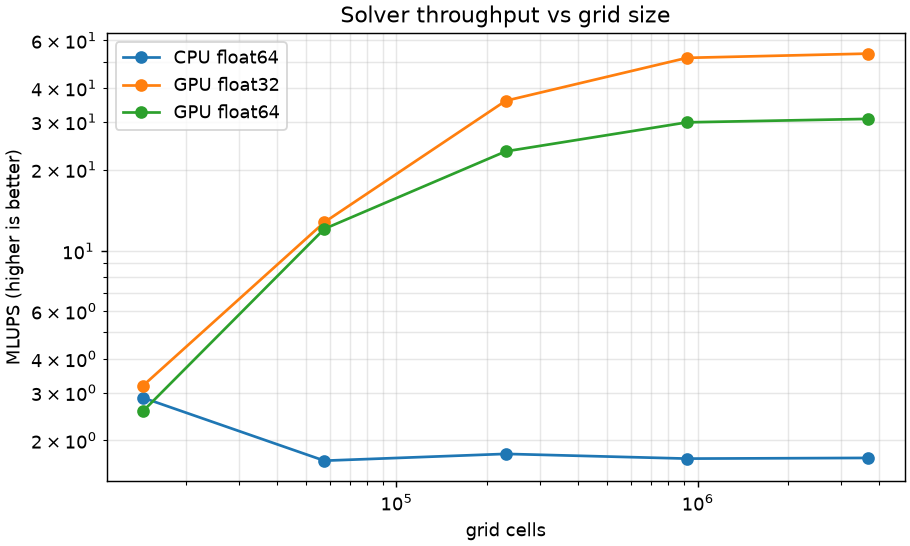
\includegraphics[width=0.7\textwidth]{scaling_grid.png}
\caption{Throughput against grid size.}\label{fig:gpu}
\end{figure}

\paragraph{Cluster.} SLURM scripts are provided for a full node, a job array (one case per task) and a GPU node. They call commands that were tested locally, but \textbf{the scripts were never run on a cluster} because no access was available.

%--------------------------------------------------------------------
\section{Discussion and limitations}\label{sec:limits}
\begin{itemize}
  \item \textbf{Simulated data.} Conclusions about real flows cannot be drawn from this benchmark. The solver is only partly validated (Strouhal number 6 to 16\% too high), and drag and grid convergence were not checked. The confinement and periodic boundaries bias the flow compared with an unbounded cylinder.
  \item \textbf{One narrow task}: 2D laminar flow, one geometry, one parameter, mean field only; no unsteady prediction, pressure, turbulence or 3D.
  \item \textbf{Modest test sets} (15 and 6 cases from one smooth family); differences of a few percent between models should not be over-interpreted. Each performance number is a single measurement.
  \item \textbf{Small baselines.} No convolutional network, U-Net or neural operator, which are the models a benchmark is ultimately meant for; the six training fields are too few to train them.
  \item \textbf{The web platform is a prototype}: no accounts, in-memory rate limit, SQLite on a single process, and anyone can tune predictions on the public test Reynolds numbers.
  \item \textbf{Modest HPC part}: one laptop, no profiling, no MPI or multi-GPU, poor CPU scaling, SLURM scripts not run on a cluster.
\end{itemize}

%--------------------------------------------------------------------
\section{Conclusions and future work}
A complete benchmarking pipeline was built and tested: dataset, solver, preprocessing, metrics, baselines, leaderboard and web platform, with continuous integration and a container image. On the proposed task, simple interpolation is hard to beat between training points, and extrapolation in the Reynolds number is the discriminating test, which justifies a dedicated split. The performance study shows that the CPU data generation is limited by memory rather than by cores, and that a GPU is only worthwhile on large grids.

Future work, in order of expected value:
\begin{enumerate}
  \item add experimentally validated and published datasets (PIV, FDA benchmarks, CFDBench, FlowBench) through the same dataset interface, and validate the solver further (drag, grid convergence, wider domain);
  \item add deep-learning baselines (CNN, U-Net, Fourier neural operator) trained on GPU;
  \item broaden the task: several geometries and parameters, unsteady prediction, pressure and vorticity, physically motivated metrics;
  \item speed up the generation: solve all Reynolds numbers as one batch on the GPU, fuse temporaries into custom kernels, then decompose large domains across several GPUs with MPI, and run the SLURM scripts on a cluster;
  \item harden the platform: authentication, persistent rate limiting, a job queue for evaluation and a production database.
\end{enumerate}

%--------------------------------------------------------------------
\appendix
\section{Reproducing the results}
\begin{lstlisting}
git clone https://github.com/Gotrone/TFM.git && cd TFM
python -m venv .venv && .venv\Scripts\activate
pip install -e ".[dev]"
pytest                      # 24 tests
cfdbench benchmark --reset  # baselines, leaderboard, figures
cfdbench scaling            # performance studies
cfdbench serve              # web platform on http://127.0.0.1:8000
\end{lstlisting}
The dataset is committed (\texttt{data/cylinder\_flow.npz}); \texttt{cfdbench generate} regenerates it (about half an hour on the machine used here).

\section{Submission format}
A submission is an \texttt{.npz} file with the arrays \texttt{test\_interp} and \texttt{test\_extrap}, each of shape $(N,2,n_x,n_y)$, channels $(u,v)$, samples in ascending Reynolds order.

\newpage
\begin{thebibliography}{9}
\bibitem{luo2023cfdbench} Y.~Luo et al. \emph{CFDBench: A Large-Scale Benchmark for Machine Learning Methods in Fluid Dynamics}. arXiv, 2023.
\bibitem{tali2024flowbench} R.~Tali et al. \emph{FlowBench: A Large Scale Benchmark for Flow Simulation over Complex Geometries}. arXiv, 2024.
\bibitem{lee2019data} S.~Lee and D.~You. Data-driven prediction of unsteady flow over a circular cylinder using deep learning. \emph{Journal of Fluid Mechanics}, 879:217--254, 2019.
\bibitem{fluidfoam} FluidFoam documentation. \url{https://fluidfoam.readthedocs.io}.
\bibitem{kruger2017lbm} T.~Kr\"uger et al. \emph{The Lattice Boltzmann Method: Principles and Practice}. Springer, 2017.
\bibitem{latt2006regularized} J.~Latt and B.~Chopard. Lattice Boltzmann method with regularized pre-collision distribution functions. \emph{Mathematics and Computers in Simulation}, 72(2--6):165--168, 2006.
\bibitem{williamson1998series} C.~H.~K. Williamson and G.~L. Brown. A series in $1/\sqrt{Re}$ to represent the Strouhal--Reynolds number relationship of the cylinder wake. \emph{Journal of Fluids and Structures}, 12(8):1073--1085, 1998.
\end{thebibliography}

\end{document}
